\documentclass{article}
\usepackage[utf8]{inputenc}
\usepackage{amsmath}
\usepackage{amsfonts}
\usepackage{graphicx}

\title{Written Assignment Unit 2\\
Math 1201- College Algebra.
}
\author{Instructor - Casmir Onyeneke}
\date{September 2021}


\begin{document}

\maketitle

\section*{Question 1}
\title Linear Functions\\
In the Question we are given sets of linear equations, to determine if they are parallel, perpendicular or neither.
\begin{description}
    \item[1a.] 
    \begin{align*}
        3y+4x = 12\\ 
        -6y = 8x+1
    \end{align*}
    rearranging both equations in slope-intercept form ${y = mx +b}$ we have
    \begin{align*}
        y = -\frac{4}{3}x + 4\\ 
        y = -\frac{4}{3}x-\frac{1}{6}
    \end{align*}
    for two lines to be parallel, their slope would have to be the same, and from the equations above the two lines are parallel because \\
    ${m1=-\frac{4}{3}}$ and ${m2 = -\frac{4}{3}}$\\
    
    The graph is shown below\\
    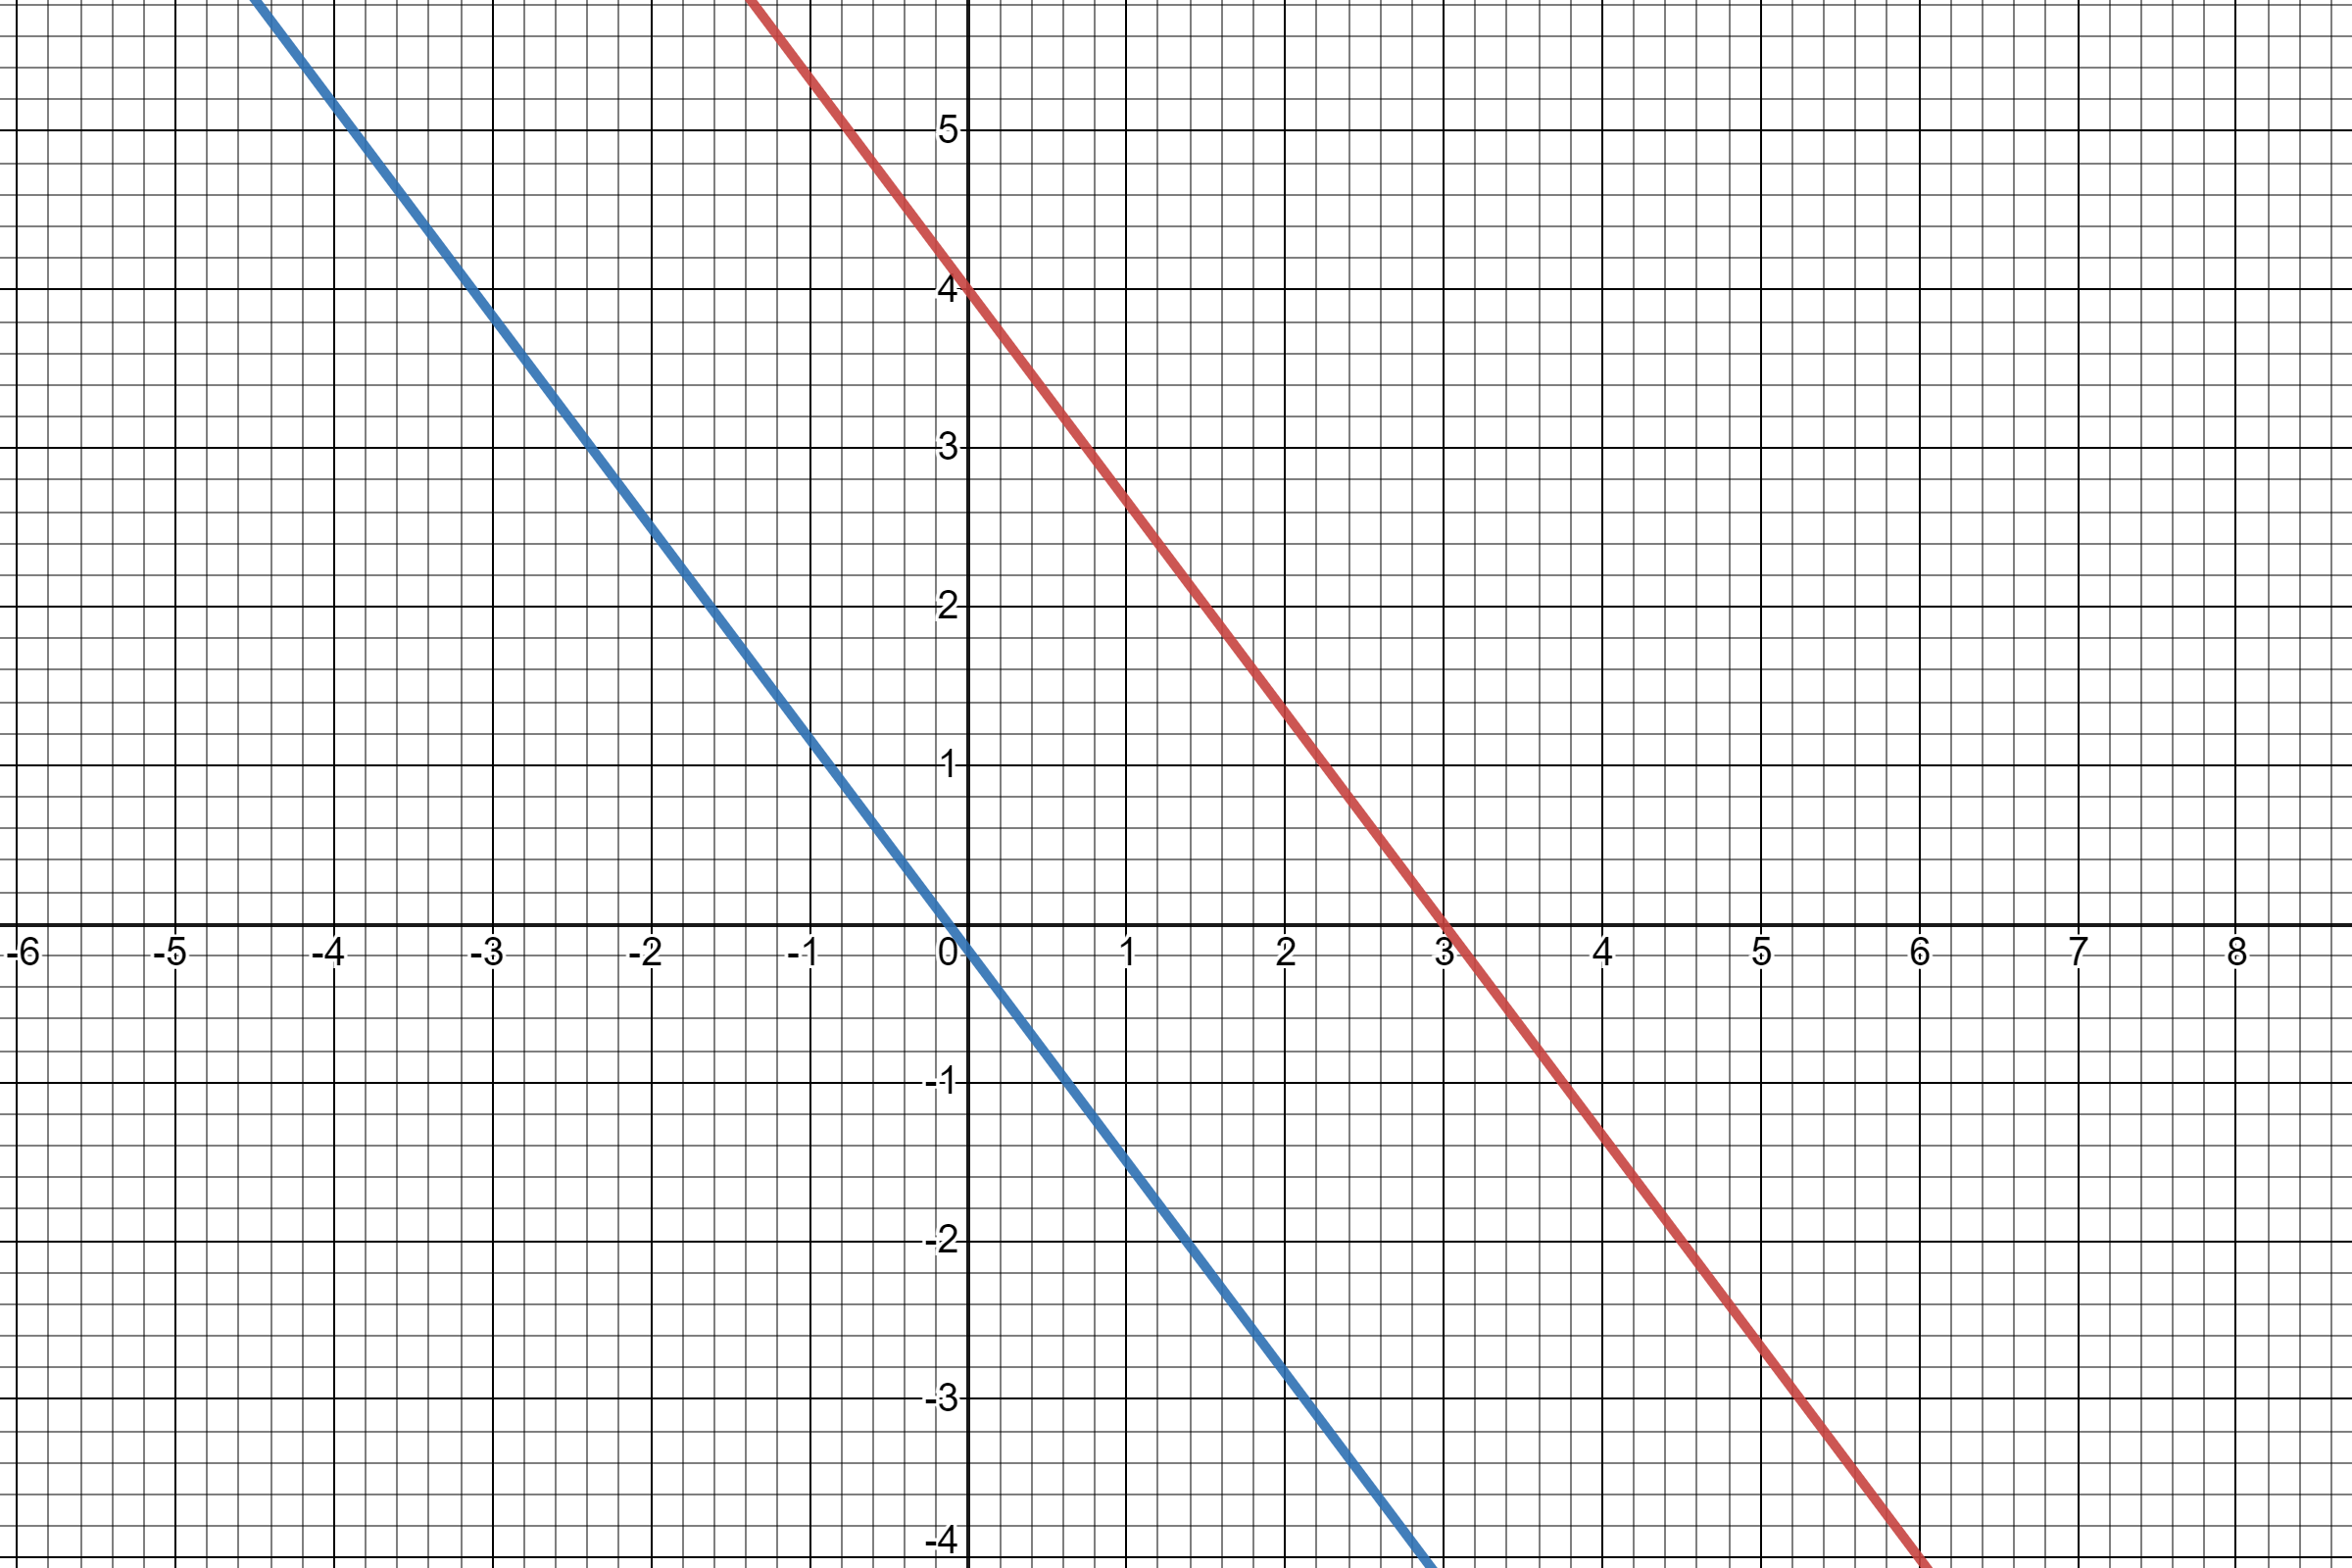
\includegraphics[scale = 0.1]{1a}
    
    
    
    
    \item [1b.]
    \begin{align*}
        3y+x = 12\\ 
        -y = 8x+1
    \end{align*}
    rearranging both equations in slope-intercept form ${y = mx +b}$ we have
    \begin{align*}
        y = -\frac{1}{3}x + 4\\ 
        y = -8x-1
    \end{align*}
    From the rearrangement we can see that both equations have different slopes and when testing for perpendicularity which requires ${m1m2=-1}$
    ${m1= -\frac{1}{3}}$ and ${m2 = -8}$
    $${-\frac{1}{3}*-8 \neq -1}$$
    Therefore we can then say that the two equations listed above are neither perpendicular or parallel.\\
    
    The graph is shown below\\
    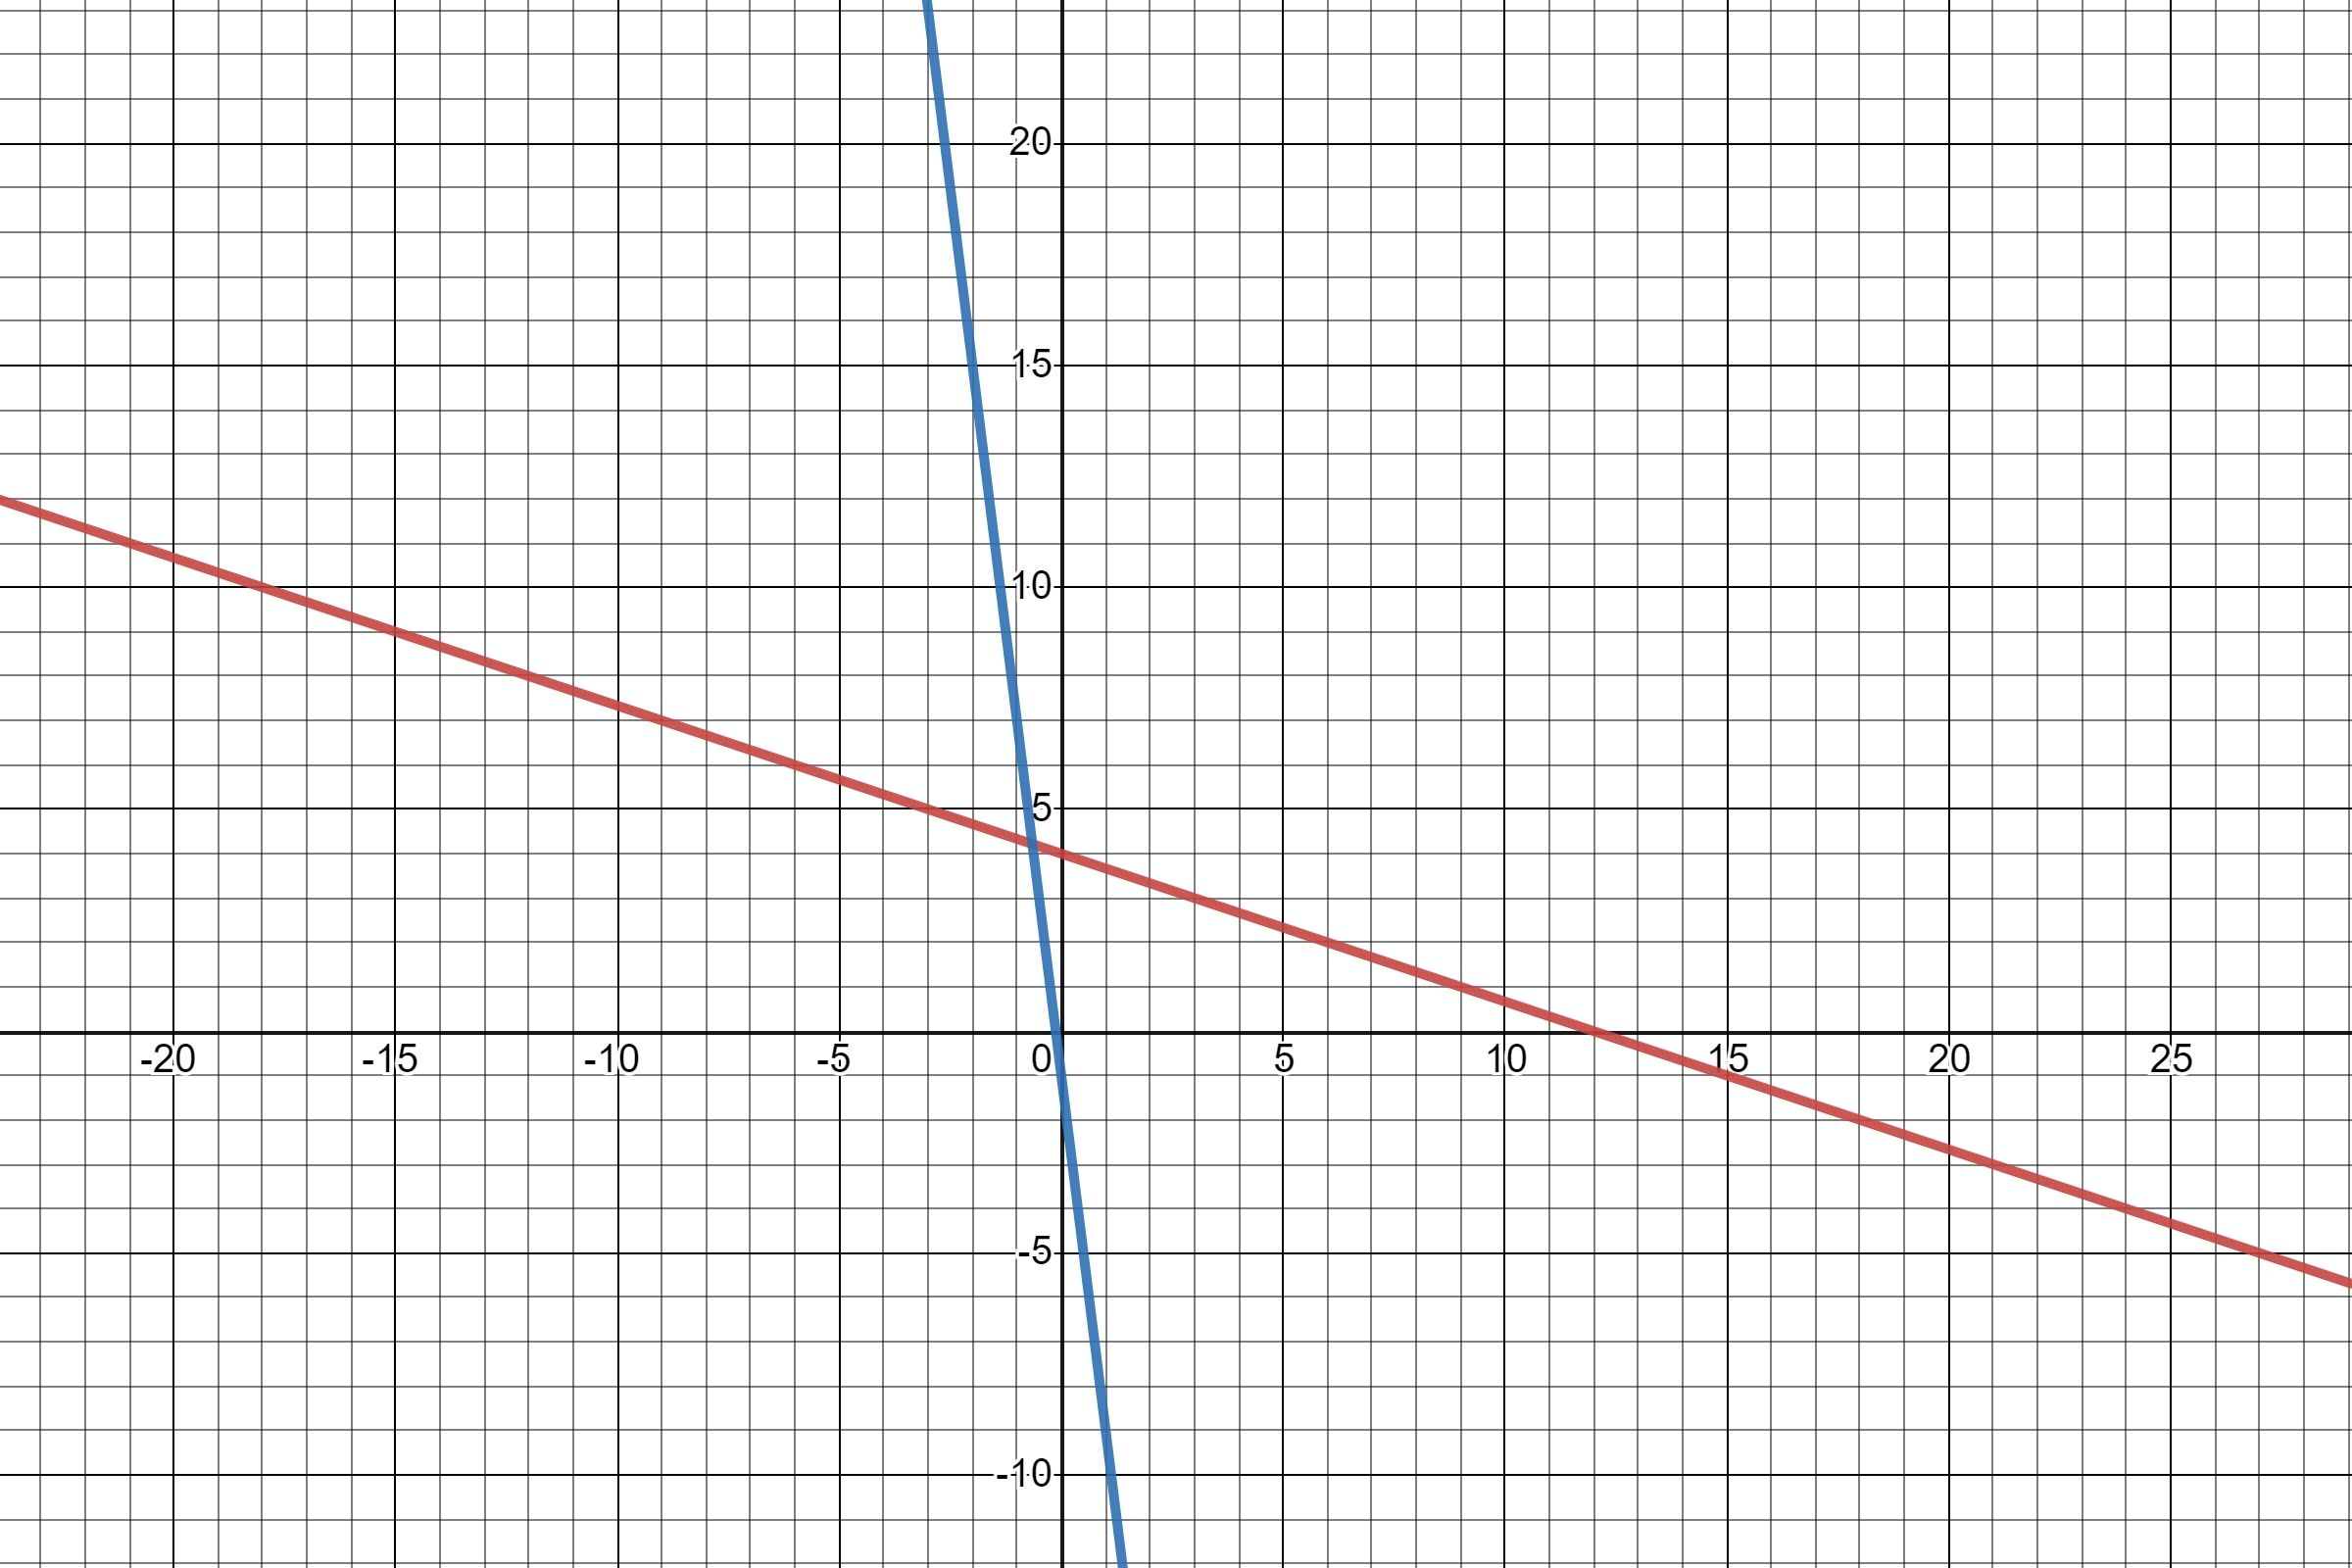
\includegraphics[scale = 0.1]{1b}
    
    
    \item [1c.]
    \begin{align*}
        4x - 7y = 10 \\ 
        7x - 4y = 1
    \end{align*}
    rearranging both equations in slope-intercept form ${y = mx +b}$ we have
    \begin{align*}
        y = \frac{4}{7}x + \frac{10}{7} \\ 
        y = -\frac{7}{4}x - \frac{1}{4}
    \end{align*}
    
    Now for two lines to be considered perpendicular$${m1=-\frac{1}{m2}}$$
    and $${m1m2=-1}$$
    solving for this we get
    $${m1=\frac{4}{7} \quad m2=-\frac{7}{4}}$$
    $${m1m2=-1}$$
    Now to check
    $${\frac{4}{7}*-\frac{7}{4} = -1}$$
    since the answer is equal to -1, we can therefore say that the two linear equations are perpendicular\\
    
    The graph is shown below\\
    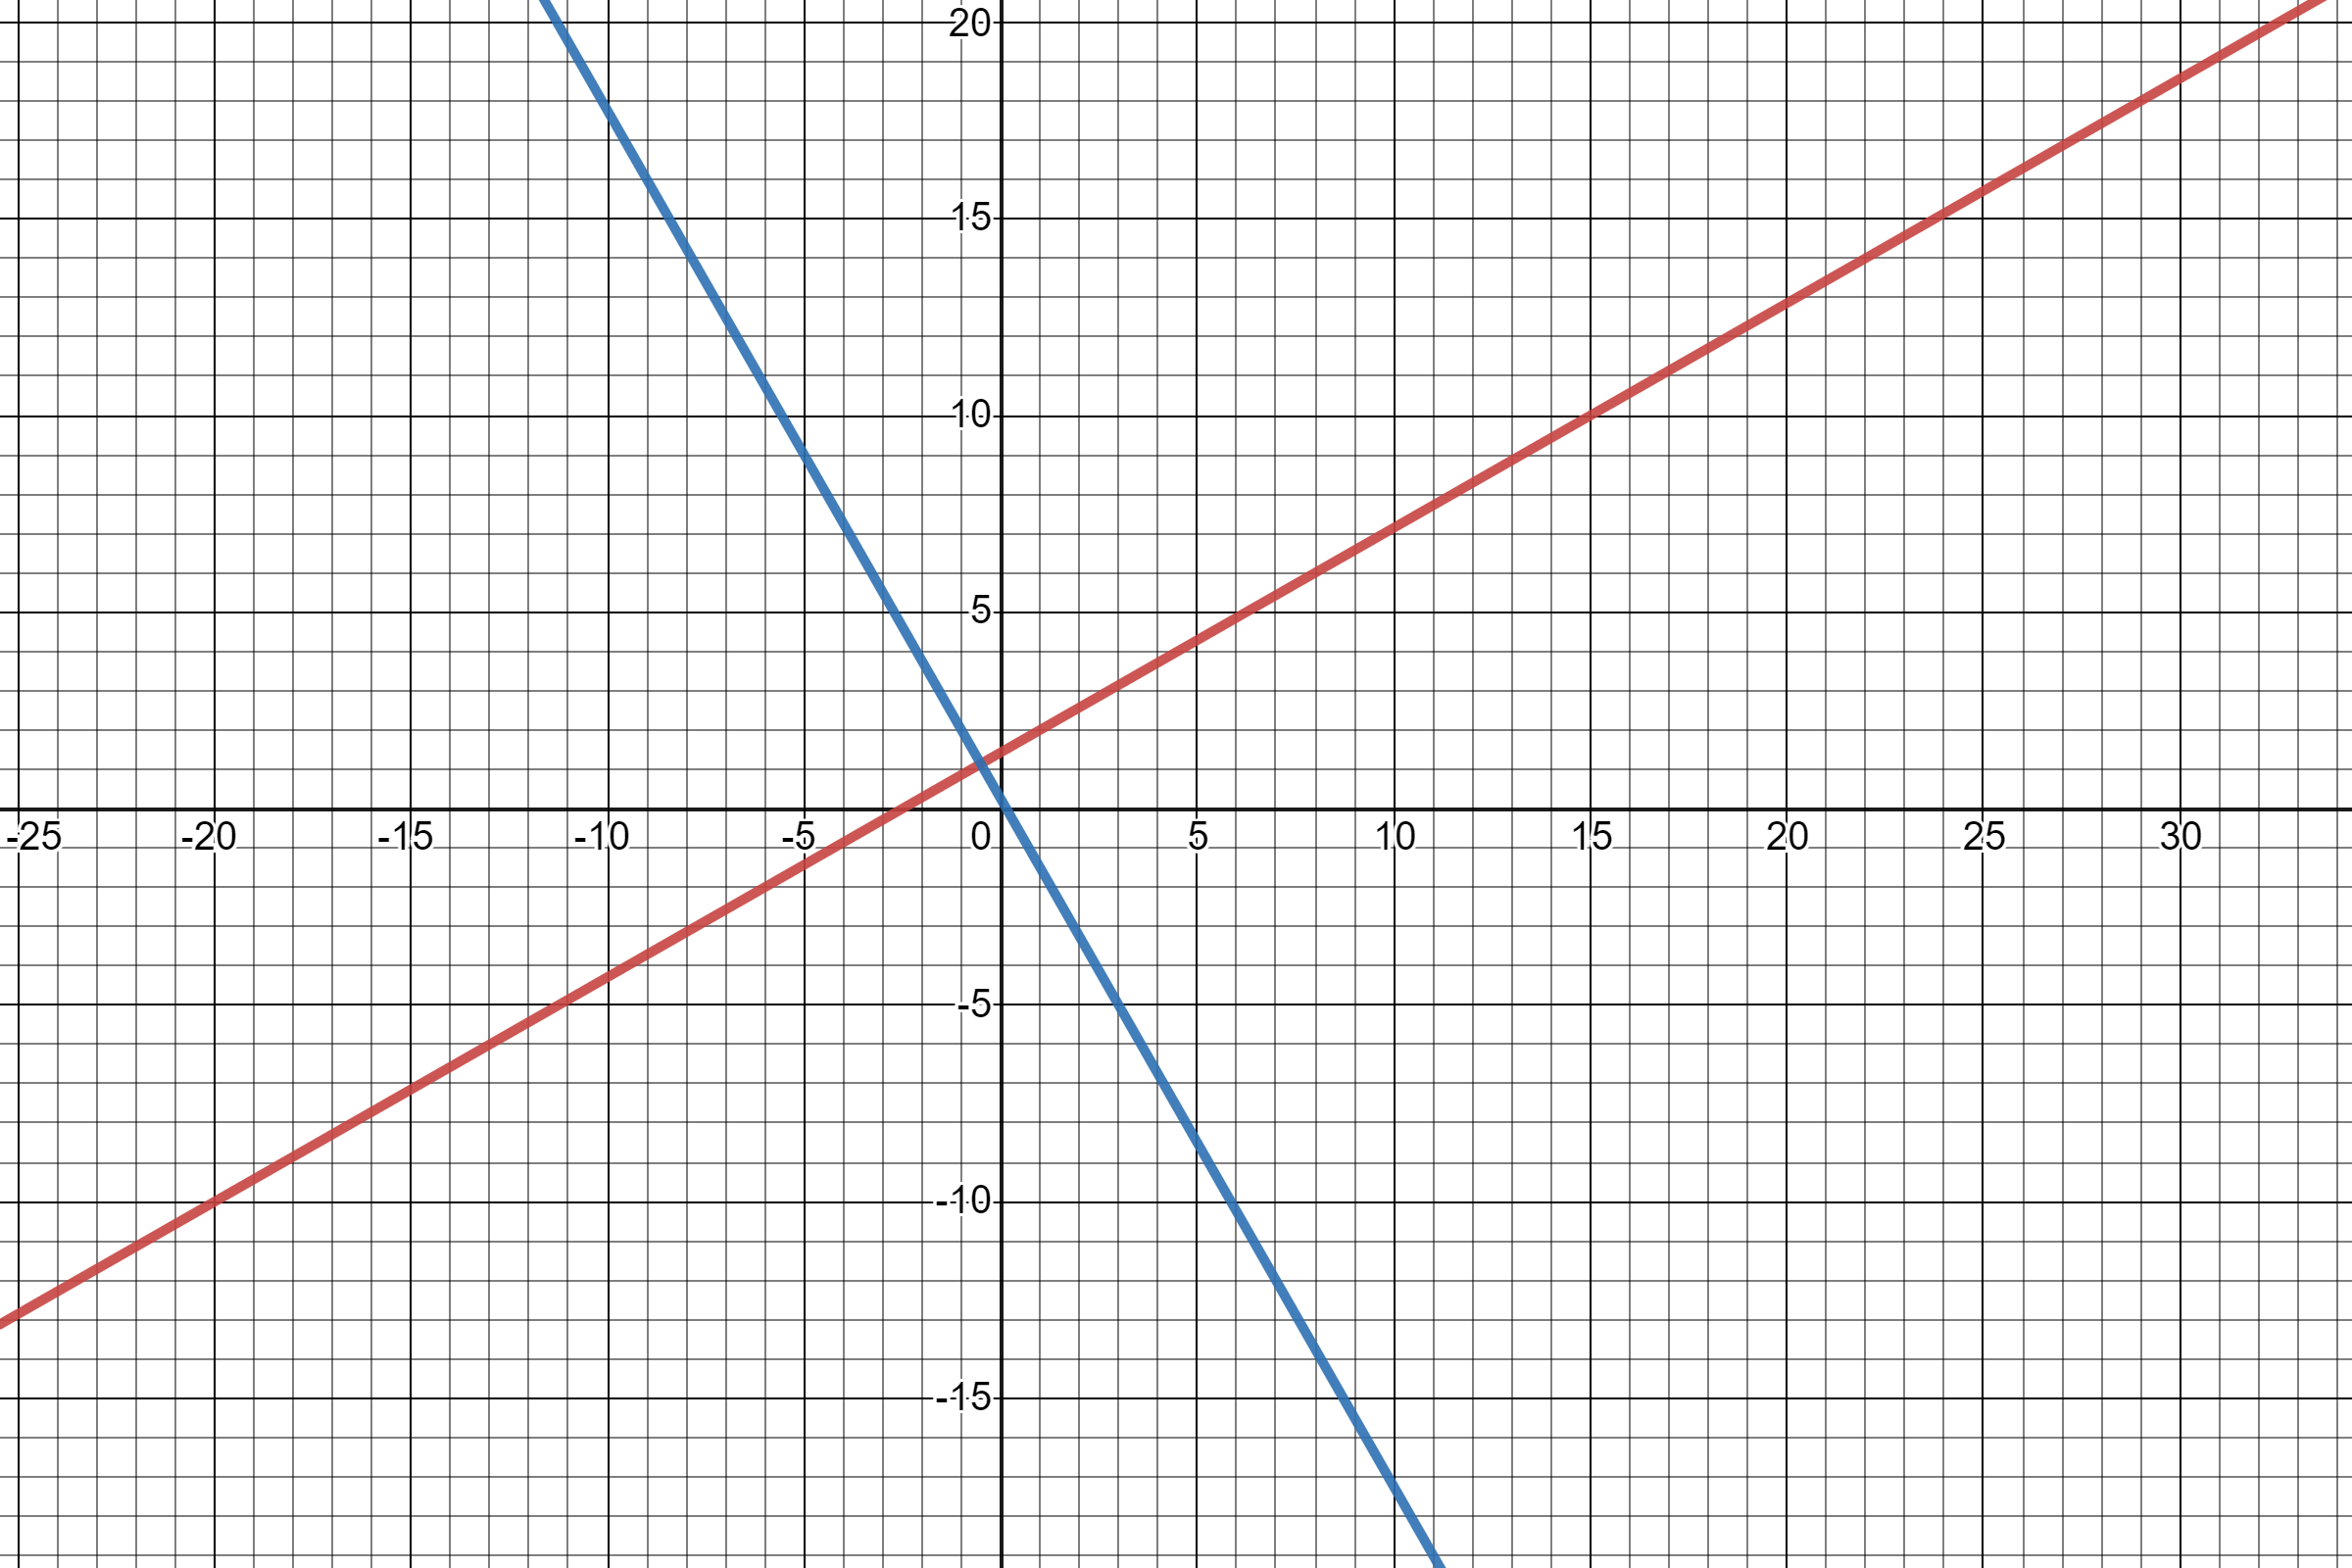
\includegraphics[scale = 0.1]{1c}
    
    
\end{description}

\section*{Question 2}
\title Quadratic Functions
So for this question the height of a building is a function of the time it takes a ball to reach the ground.\\
\begin{description}
    \item[2a.]
    The height of the building can be said to be the initial position or height of the ball when the time is zero, t, is 0.        \\
    The quadratic function is expressed as \\
    $${h(t) = 4.9x^2 +24t + 8}$$
    at t, = 0
    $${h(0)=-4.9*(0)^2 + 24*0 + 8}$$
    $${h(0)=8}$$
    Therefore the height of the building is 8 meters
    
    \item[2b.]
    The maximum height reached by the ball can be gotten from the axis of symmetry which is given by ${h=-\frac{b}{2a}}$\\
    Therefore $${h=-\frac{24}{2*-4.9}}$$
    $${h=2.4}$$
    
    $${h(2.4) = -4.9(2.4)^2+24(2.4)+8}$$
    $${h(2.4) = -28.2+57.6+8}$$
    $${h(2.4) = -37.4}$$
    Therefore the Maximum height reached by the ball is 37.4 meters.
    
    \item[2c.]
    Time it takes to reach the maximum height, can be found at the vertex of the parabola\\
    $${x=-\frac{b}{2a}}$$
    $${x=-\frac{24}{2(-4.9)}}$$
    $${x=\frac{-24}{-9.8}}$$
    $${x=2.45}$$
    
    Therefore it takes the ball 2.45 seconds to reach the maximum height.
    
    The graph is shown below\\
    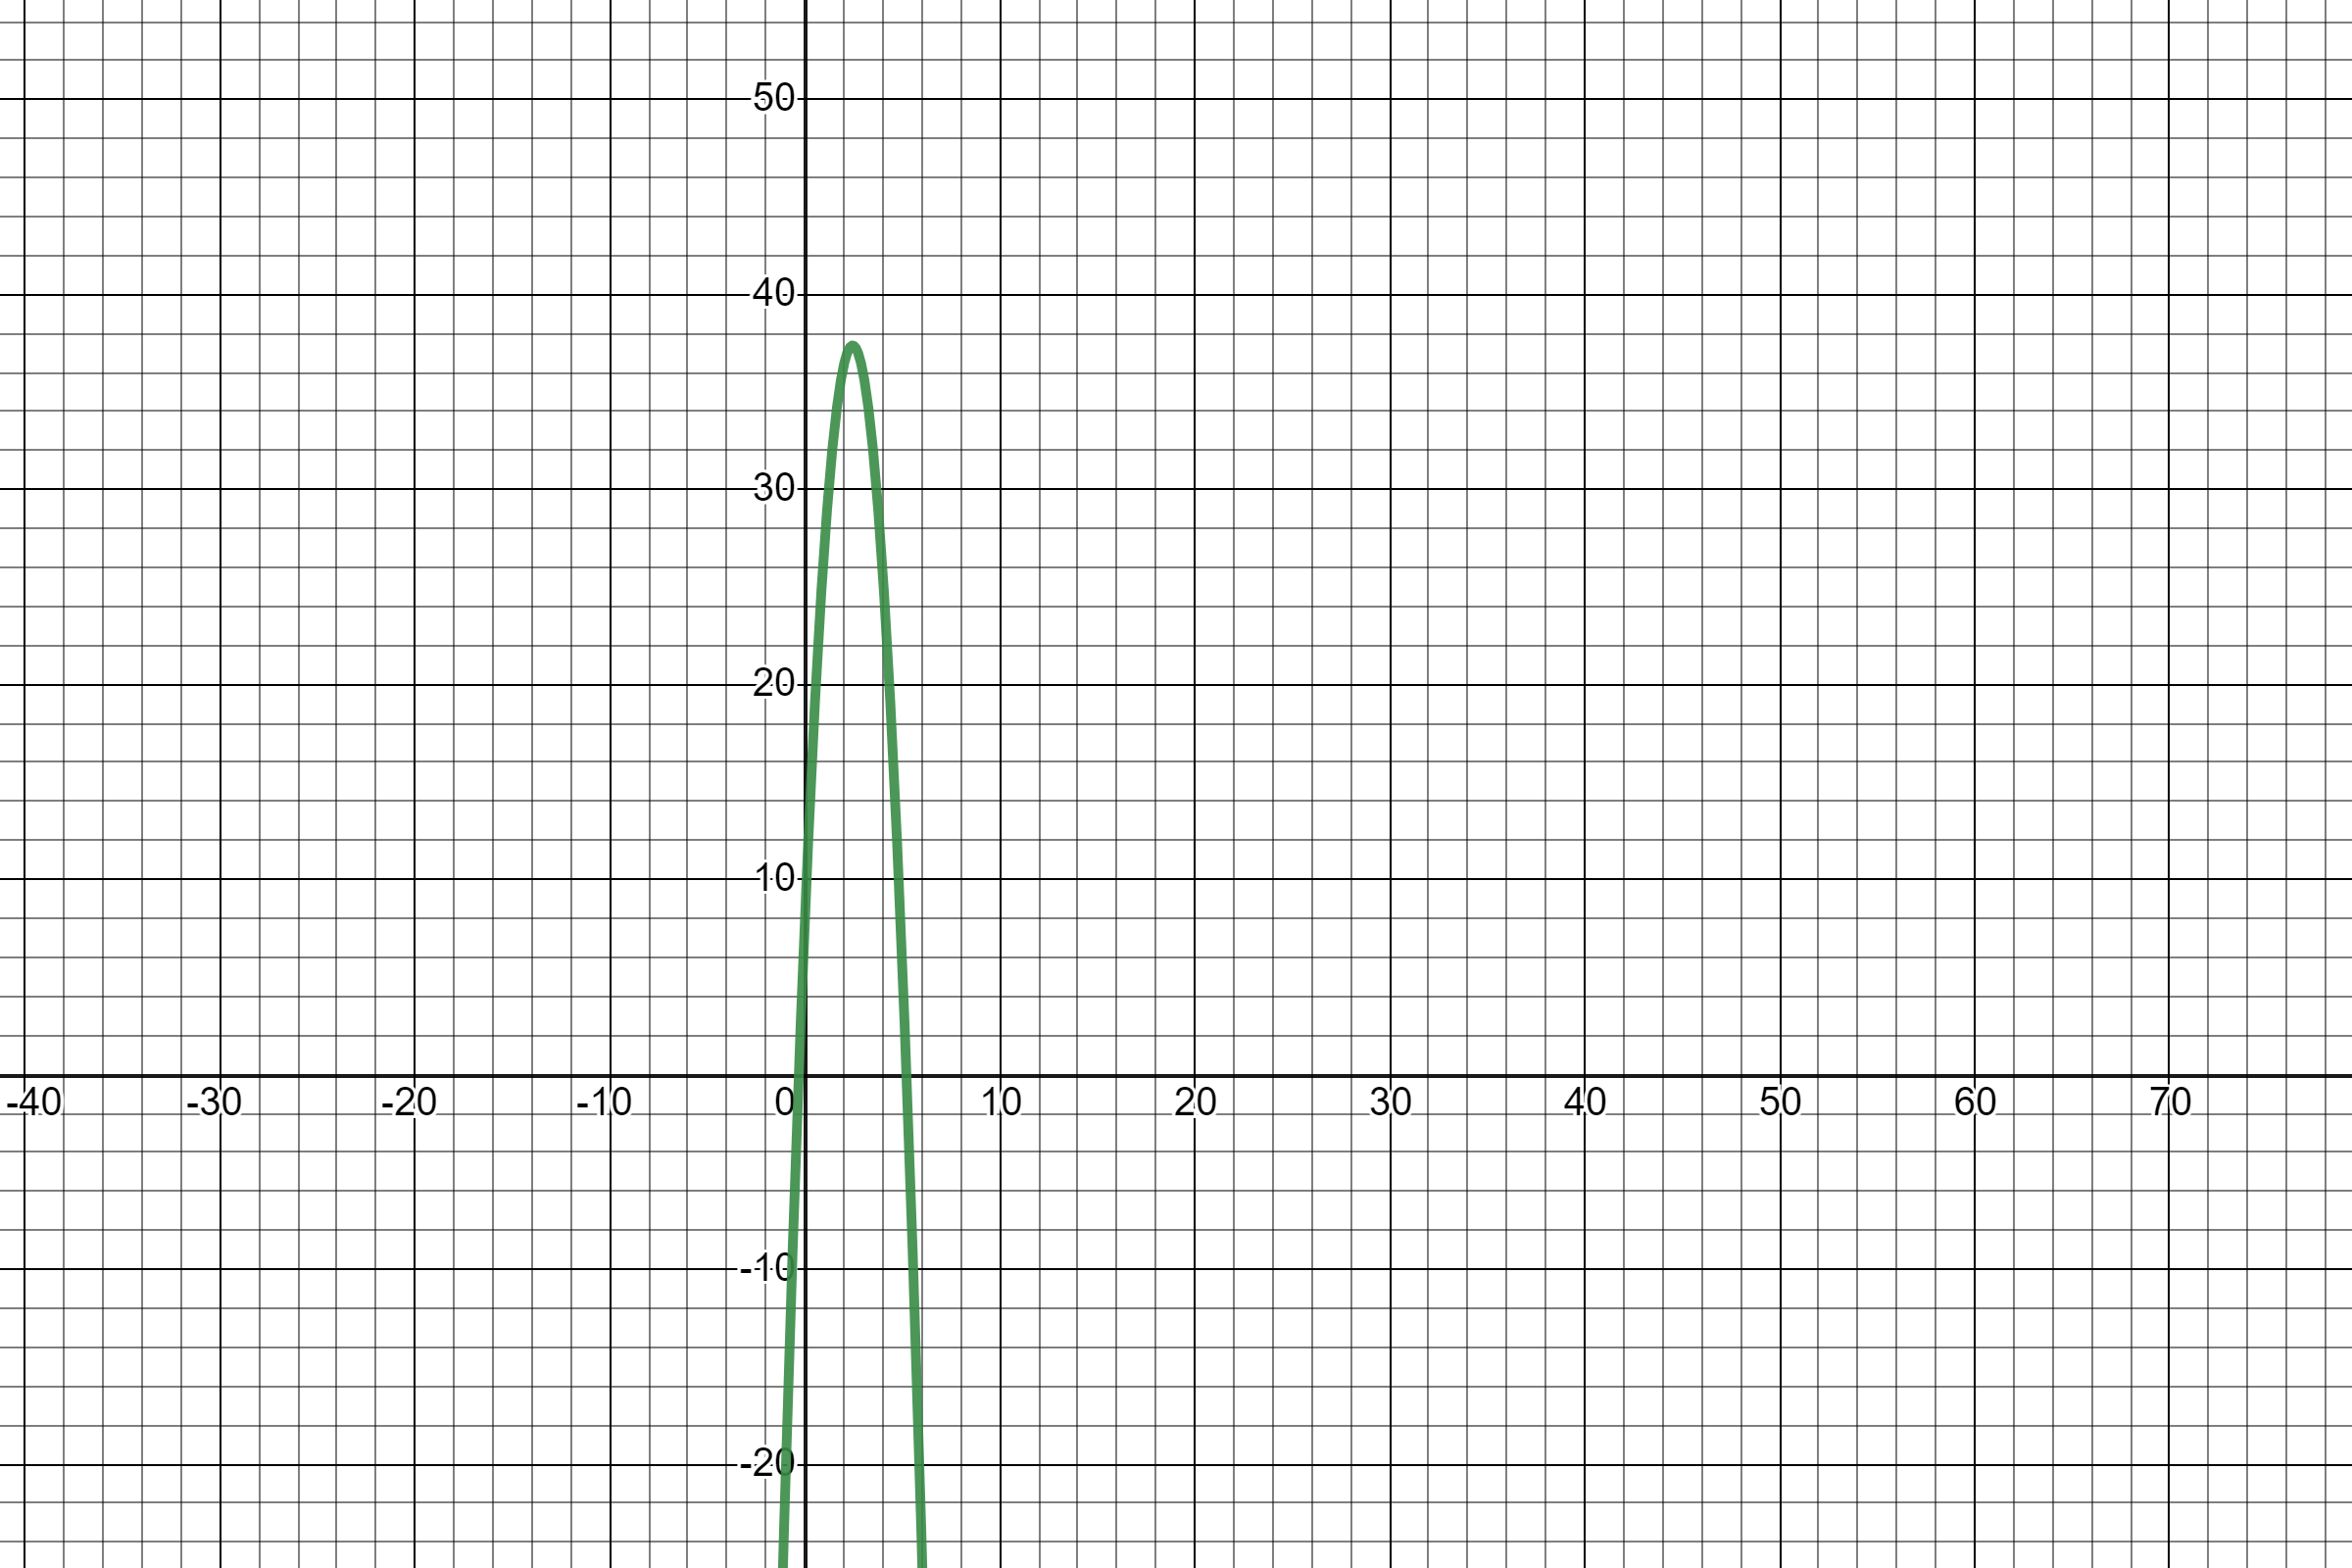
\includegraphics[scale = 0.1]{2a}
\end{description}









\section*{Question 3}
We can say that the trees are a function of the bushels, i.e 
the trees can be represented by x and the bushels by y.

from the question, $${x1=75, \quad y1=20 , \quad slope =-3 }$$
using the point-slope form to find the intercept.
$${y-y1 = m(x-x1)}$$
$${y-20 = -3(x-75)}$$
$${y = -3x+225+20}$$
$${y = -3x + 245}$$

Our function B(n) = xy
Therefore to find how many trees per acre, would need to be planted in order to maximize the harvest of the farmer, we would have to evaluate B(n). 
$${B(n)=xy}$$
$${B(n)= x(-3x + 245) }$$
$${B(n)= -3x^2 + 245x}$$
The maximum harvest is given by the vertex of the curve.
$${Max= -\frac{b}{2a},\quad a=-3, \quad b=245, \quad c = 0}$$
$${Max= \frac{-245}{-2(3)}}$$
$${Max= \frac{-245}{-6}}$$
$${Max = 40.83}$$
$${Max \approx 41}$$
Therefore approximately the farmer would need to plant 41 trees in order to maximize her harvest

The graph is shown below\\
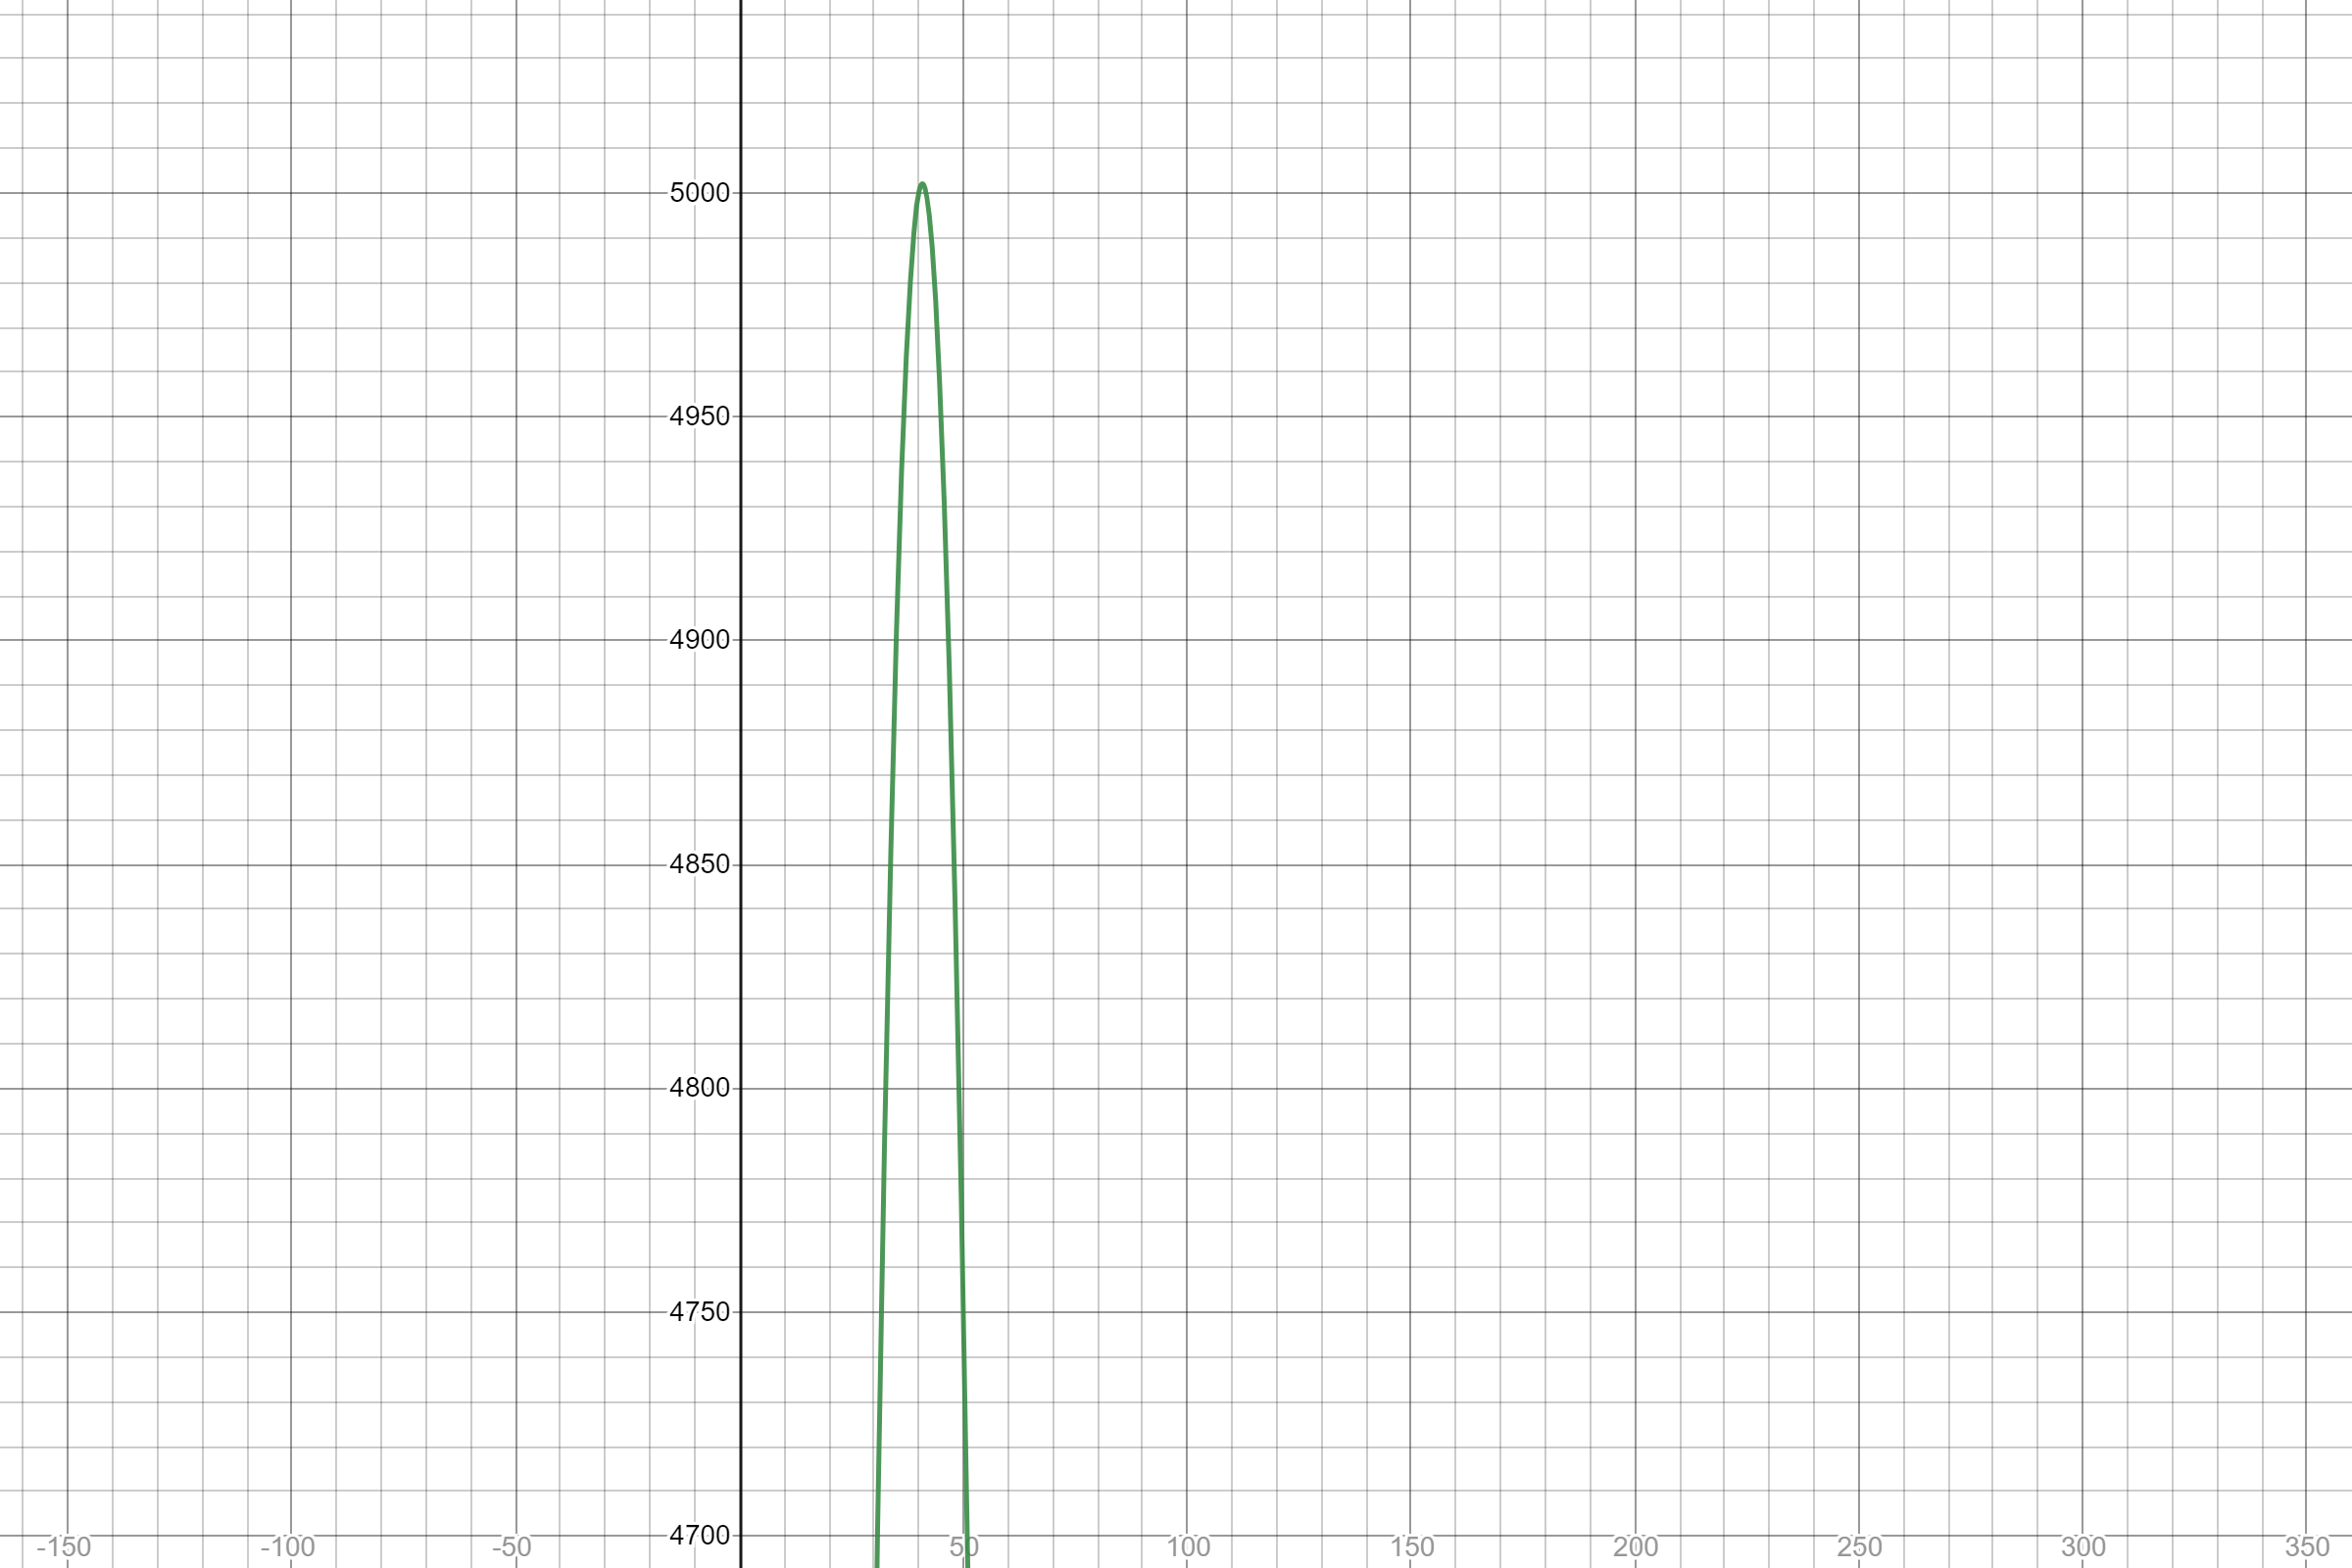
\includegraphics[scale = 0.1]{3b}

\section*{References}
Abramson, J. (2017). \textit{Algebra and trigonometry}. OpenStax, TX: Rice University. Retrieved
from https://openstax.org/details/books/algebra-and-trigonometry
\end{document}
